\chapter{HpCom: A Data Mining and Optimization Platform for Optical Communication}

\section{Introduction}
In the rapidly evolving field of optical communication systems, researchers face increasingly complex problems and large-scale computations. The need for efficient and high-performance simulation tools is paramount. While there are established simulation methods, there is currently a gap in the availability of high-performance software tailored to the unique requirements of optical communication systems. This paper aims to address this gap by introducing a GPU-accelerated framework -- High-Performance COMmunication library\cite{esf0_2023_7880552}, designed to enhance simulation capabilities and accelerate innovation in the field.

The use of GPU-based implementations in optical communication system simulations offers several key advantages over traditional CPU-based methods\cite{brehler2017gpu}. One of the primary benefits is the inherent parallelism in GPU architectures. With thousands of cores capable of handling multiple operations simultaneously, GPUs are better suited for the parallel computations often found in optical communication system simulations. This leads to improved performance, particularly for tasks involving large-scale matrix operations, vector manipulations, or Fourier transforms.

Scalability is another significant advantage of GPU implementations, as they can be more easily adapted to handle larger problem sizes or more complex simulations. This flexibility is crucial for researchers working on cutting-edge optical communication systems, as computational demands continue to grow.

Moreover, GPUs are known for their power efficiency in parallel computations. For large-scale simulations, using GPUs can result in considerable energy savings compared to CPU-based implementations. This is particularly important when generating vast amounts of data for machine learning techniques or tackling high-dimensional optimization problems\cite{srivallapanondh2022knowledge, genty2021machine, reznichenko2022optimal}.

The accelerated computation offered by GPUs enables researchers to rapidly test hypotheses\cite{winzer2012optical}, iterate on designs, and explore a wider range of scenarios in a shorter amount of time. This results in faster discovery of new insights and innovations, as well as more efficient use of resources for data analysis, interpretation of results, and further development of novel techniques.

\begin{figure}[t]
   \centering
        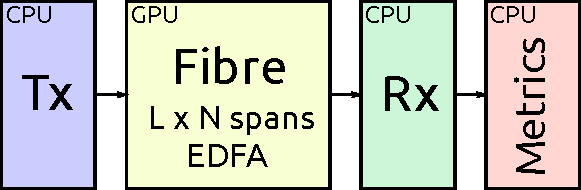
\includegraphics[width=0.8\linewidth]{images/hpcom/hpcom_scheme.pdf}
    \caption{Framework architecture for optical communication system simulation, featuring optimized transceiver (Tx) design, GPU-accelerated SSFM-based channel model (with $N$ spans of length $L$), receiver implementation (Rx), and performance metrics evaluation including BER, EVM, and MI.}
    \label{fig:hpcom_scheme}
\end{figure}

By filling the current gap in high-performance software for optical communication system simulations, our GPU-accelerated framework has the potential to transform research in the field. Its user-friendly design, combined with its powerful capabilities, allows researchers to focus on their novel tasks rather than being constrained by well-established simulations. This paper provides an in-depth overview of the framework's architecture, highlighting its benefits and showcasing its potential for driving new discoveries in optical communication systems.

\begin{figure*}[t]
   \centering
    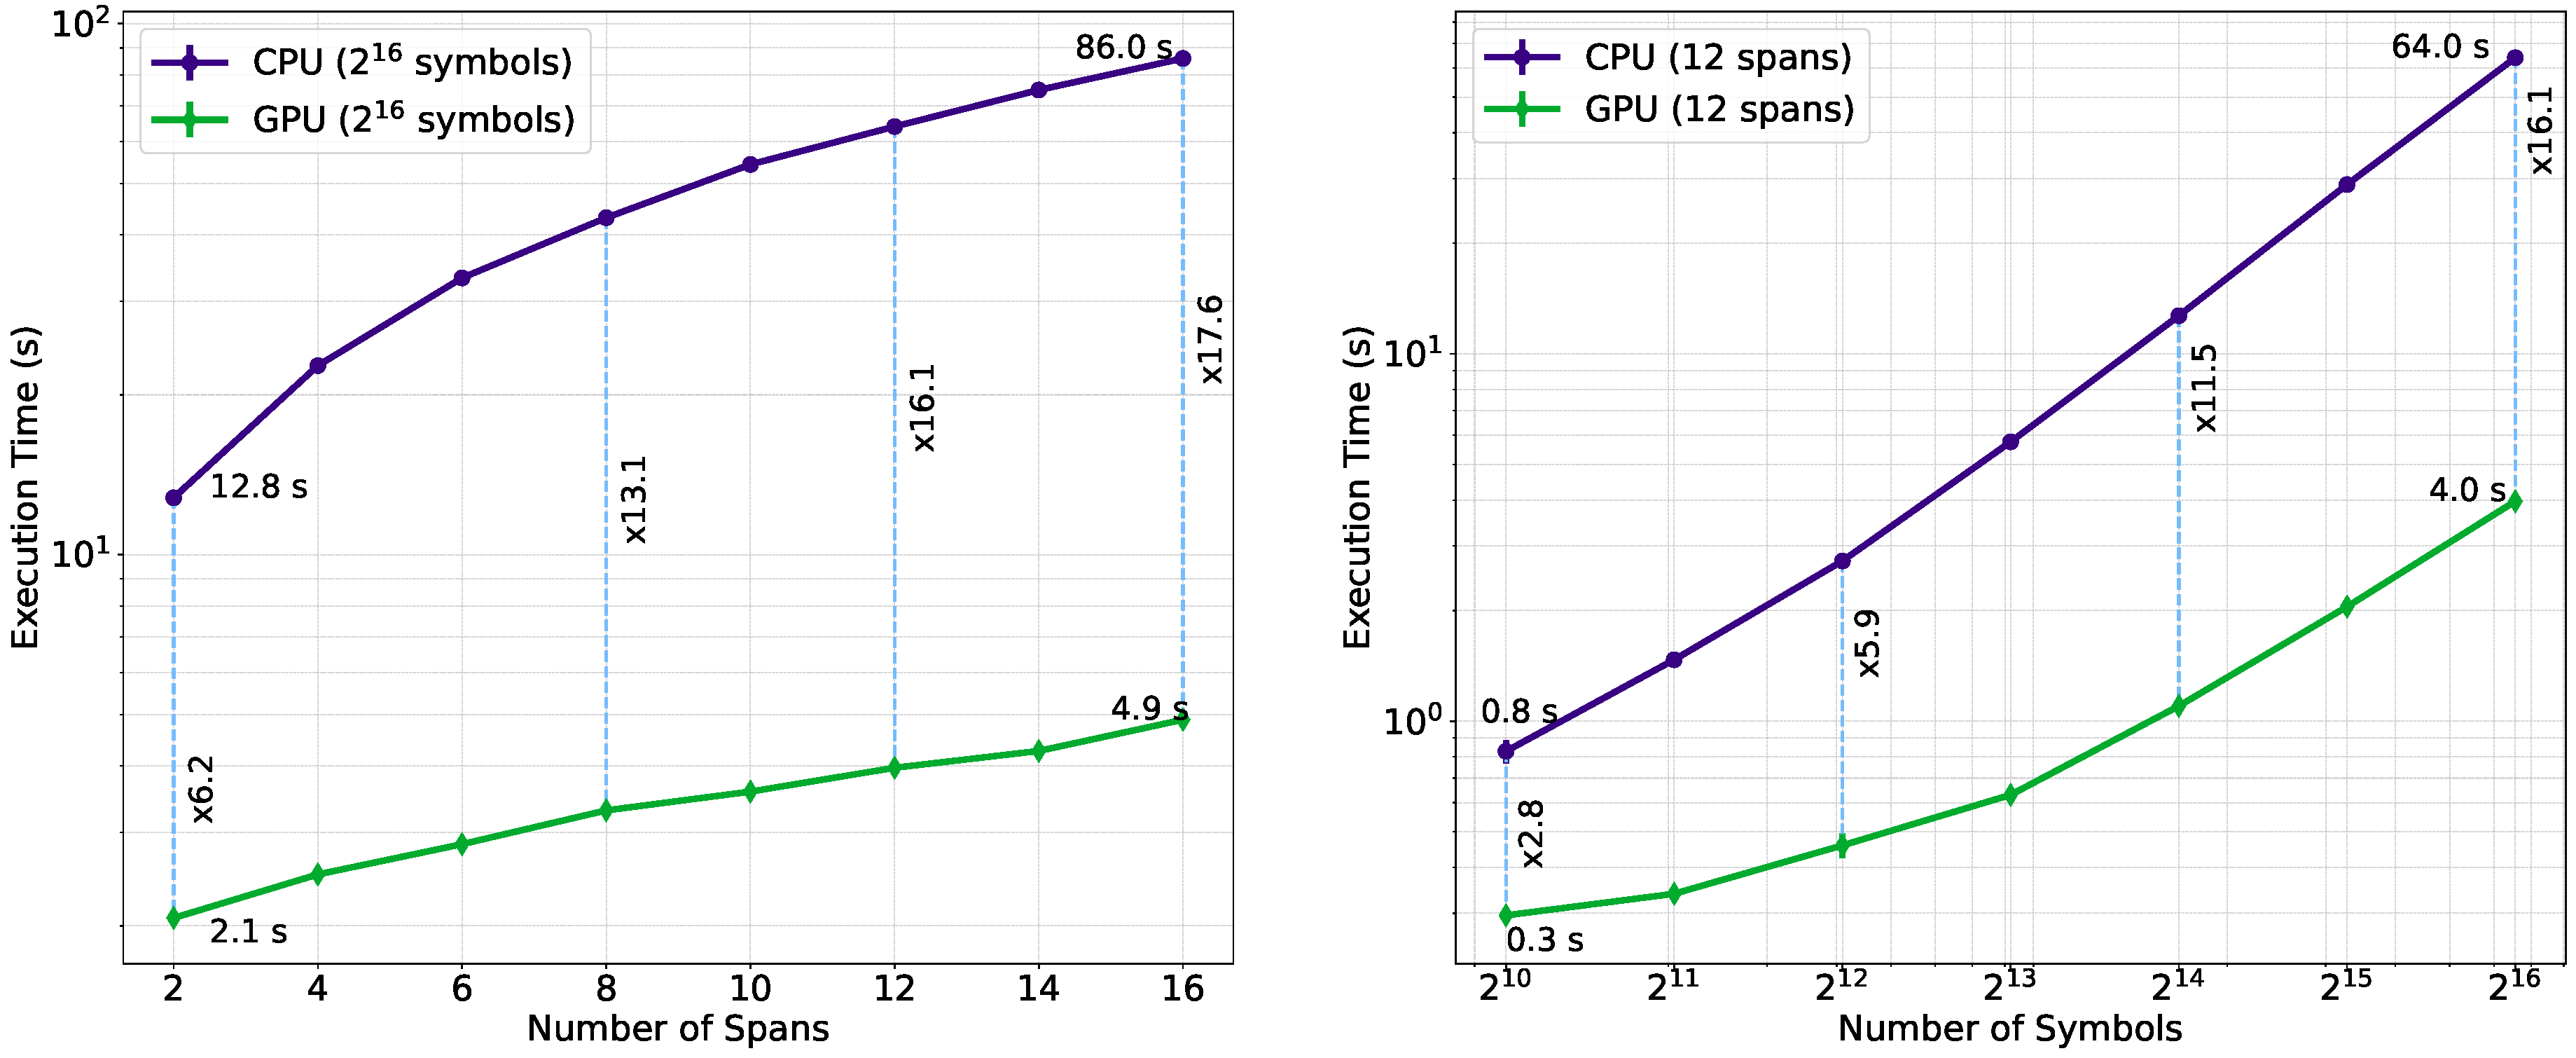
\includegraphics[width=1\linewidth]{images/hpcom/total.pdf}
    \caption{The left figure displays the total execution time for all steps of the optical channel simulation with $2^{16}$ symbols, comparing single CPU core and GPU usage, as a function of the number of spans (SMF, each span is 80 km). The right figure illustrates the relationship between execution time for a single CPU core and GPU usage with a fixed number of spans and varying number of symbols in the simulation.}
    \label{fig:total}
\end{figure*}


\section{Framework Architecture and Methodology}
The proposed framework is built on the TensorFlow 2.x library, with Python as the primary programming language. It is designed to be compatible with the MATLAB environment through the \textrm{pyrun} function, enabling seamless integration with existing MATLAB workflows.

The main components of the framework include the transmitter (Tx), the optical channel model (using SSFM and its higher-order variations), the receiver (Rx), and the metrics evaluation block (see Fig.~\ref{fig:hpcom_scheme}). By default, the transmitter generates a WDM signal with properties as described below. Once the signal is formed by the Tx, it is passed to the second block - the channel model, where a standard single-mode fiber (SSFM) optical channel is simulated with variable numbers of spans and an Erbium-Doped Fiber Amplifier (EDFA) scheme. The Rx consists of a matched filter implementation, chromatic dispersion compensation (CDC), signal demodulation and hard decision blocks. After processing the received information, it can be used to evaluate desired performance metrics such as Bit Error Rate (BER), Error Vector Magnitude (EVM), Mutual Information (MI), or any custom metric.

The Schr\"odinger equation and the Manakov equation are two widely-used mathematical models that describe light propagation in single-mode optical fibers, taking into account dispersion and nonlinearity effects\cite{agrawal2000nonlinear}. The Schr\"odinger equation models the evolution of the slowly varying optical field envelope, while the generalized Manakov equation provides a more sophisticated model for light propagation in a two-polarization optical fiber, including polarization-mode dispersion and nonlinear interactions between polarizations\cite{poletti2008description, mumtaz2012nonlinear}.

Our framework incorporates both of these models, utilizing a GPU-accelerated SSFM implementation for the efficient and accurate simulation of optical communication systems. This forms the core of the framework, ensuring that it can handle complex scenarios and deliver reliable results. Further details on the implementation can be found in the accompanying framework documentation\cite{esf0_2023_7880552}.

By default, our framework employs a classical WDM channel scheme for SSMF with an EDFA\cite{essiambre2010capacity}, and ideal transmitter and receiver. However, users can easily customize their channel line by adjusting various parameters for the simulations. For instance, you can explore other types of optical fibers such as TrueWave Classic\cite{taylor2002application} (TWC) or Large Effective Area Fiber\cite{charlet200972} (LEAF) with corresponding parameters. Additionally, you can modify signal parameters to use not only WDM with Quadrature Amplitude Modulation (QAM) but also other types of modulations or signals.

The default model can be further customized using internal framework functions, for example, by adding noise to the transmitter to simulate the imperfections of real systems.

Main WDM parameters include:
\begin{itemize}
     \item  \textrm{n\_channels}: number of WDM channels,
     \item  \textrm{p\_ave\_dbm}: signal average power in dBm,
     \item  \textrm{n\_symbols}: number of symbols in the signal,
     \item  \textrm{m\_order}: order of the modulation format,
     \item  \textrm{roll\_off}: roll-off factor for the RRC filter,
     \item  \textrm{upsampling}: upsampling factor,
     \item  \textrm{symb\_freq}: symbol frequency,
     \item  \textrm{channel\_spacing}: WDM channel spacing,
     \item  \textrm{n\_polarisations}: number of polarizations.
\end{itemize}

Main channel parameters include:
\begin{itemize}
     \item  \textrm{n\_spans}: number of fiber spans in the system,
     \item  \textrm{z\_span}: length of each fiber span in km,
     \item  \textrm{alpha\_db}: fiber attenuation in dB/km,
     \item  \textrm{gamma}: fiber nonlinear coefficient in W$\cdot$km,
     \item  \textrm{noise\_figure\_db}: EDFA noise figure in dB,
     \item  \textrm{dispersion\_parameter}: fiber dispersion parameter in ps/(nm$\cdot$km),
     \item  \textrm{dz}: step size in km for the fiber propagation.
\end{itemize}

\section{Performance Evaluation}
To evaluate the framework's performance, we conducted several tests comparing computation time between CPU and GPU. The signal used was a two-polarization 64-QAM WDM with 1 km per step and 80 km span. The SSMF fiber parameters were: $\gamma$ = 1.2 (W$\cdot$ km)$^{-1}$, $D$ = 16.8 ps/(nm$\cdot$km), and $\alpha$ = 0.21 dB/km. At the end of each span, optical fiber losses were compensated using an EDFA with a 4.5 dB noise figure. The benchmark calculations were performed using an NVIDIA GeForce RTX 3070 with 8GB GDDR6 and a single core of an AMD Ryzen 9 5900HX with up to 4.6GHz.

The total simulation time consists of four components: the transmitter (Tx) simulation time $T_{Tx}$, channel simulation time $T_{channel}$, receiver (Rx) simulation time $T_{Rx}$, and metrics evaluation time $T_{metrics}$. In the current implementation, Tx, Rx, and metrics calculations utilize CPU cores, but employ optimized functions to prevent $O(n^2)$ computational complexity. For instance, with $2^{15}$ symbols, Tx, Rx, and metrics calculations take approximately 200 ms, significantly less than the propagation time (1230 ms for GPU and 27000 ms for CPU). Optimal results are observed when working within the available GPU memory. When the number of simulation points equals $\mathrm{n\_symbols} \cdot \mathrm{upsampling} = 2^{16} \cdot 2^{4}$, the overall memory required for calculations is around 6.5 GB. To perform more precise simulations for multi-channel WDM signals, one must control the overall number of points or employ more advanced hardware.

Figure~\ref{fig:total} displays the dependence of total execution time on the number of spans for a fixed number of symbols (left), and the dependence of total execution time on the number of symbols with fixed propagation length (right). The graphs indicate that as the number of spans or symbols increases, the GPU's speedup factor also grows. For instance, for $2^{16}$ symbols and 16 spans, the GPU is 17 times faster.

We also evaluated the system performance for an extreme case, where the total memory required significantly exceeds the GPU's capacity. We conducted simulations with $2^{19}$ symbols (eight times more memory than the current GPU) and separately assessed the time for each component of the simulations (Fig.~\ref{fig:propagation_time}). The graph demonstrates that the gain is independent of the propagation length, as expected, and remains approximately 34 times faster on the GPU compared to the CPU. However, for long propagation lengths (or more steps per span), the total time saved is substantial, as the GPU completes the simulation in under a minute (53.8 s), while the CPU takes over 30 minutes.

\begin{figure}[t]
   \centering
        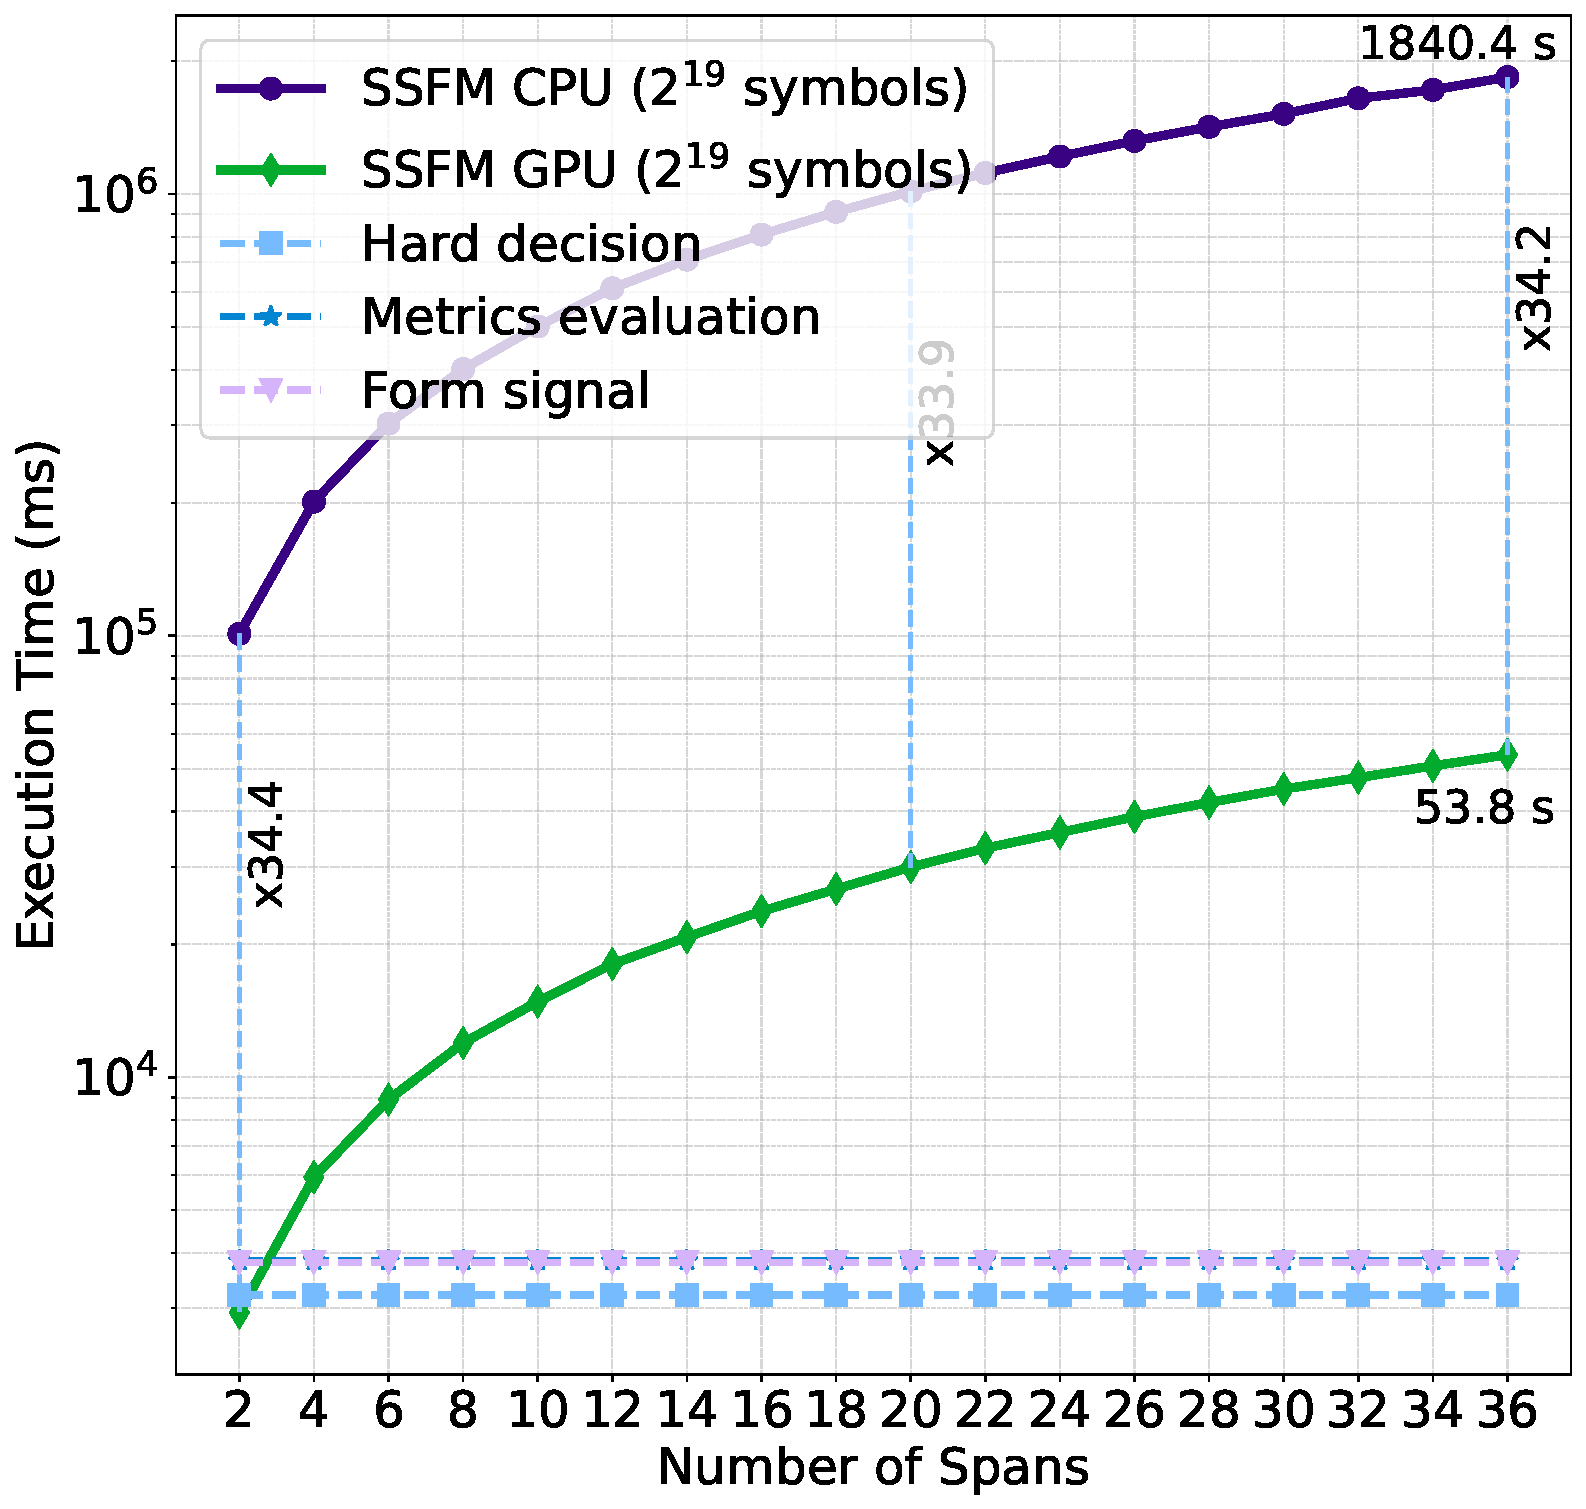
\includegraphics[width=0.7\linewidth]{images/hpcom/propagation.pdf}
    \caption{Execution time in milliseconds for various simulation steps as a function of the number of spans. Signal formation at the Tx, hard decision at the Rx, and metric evaluation (e.g., BER, EVM, MI) rely on the CPU and are influenced by the number of symbols, depicted as dashed lines. Propagation, which is performed on either the CPU or GPU, is represented by solid lines.}
    \label{fig:propagation_time}
\end{figure}

% The results were obtained by measuring the execution time of both implementations for various problem sizes (n\_symbols) while keeping the number of fiber spans (n\_spans) constant at 12. The mean execution time and standard deviation were calculated over multiple runs (7 runs for most cases) to ensure the accuracy of the results.

% Upon analyzing the graph, we observe that the GPU execution times are consistently lower than the CPU execution times across all problem sizes. Furthermore, the difference in execution times between the two implementations increases as the problem size grows, indicating that the GPU-accelerated framework becomes more advantageous for larger problems.

% Specifically, the speedup achieved by the GPU implementation relative to the CPU implementation ranges from approximately 2.8x for smaller problem sizes (n\_symbols = 2 ** 10) to around 16.1x for larger problem sizes (n\_symbols = 2 ** 16). This trend suggests that the GPU-accelerated framework is particularly well-suited for large-scale simulations or scenarios where rapid computation is required.

% In conclusion, the graph clearly demonstrates the superior performance of the GPU-accelerated framework compared to the CPU-based implementation, particularly for larger problem sizes. The increased speedup achieved with the GPU implementation highlights the benefits of utilizing GPU acceleration for optical communication system simulations.


\section{Conclusion}
The GPU-accelerated framework presents a marked improvement in performance over CPU-based implementations, especially for larger problem sizes and complex simulations. The significant speedup achieved with GPU acceleration underscores its wide-ranging benefits in various aspects of optical communication system simulations, such as advanced research, high-dimensional optimization problems, swift validation of theoretical concepts, and adjustment of simulation parameters. Moreover, the accelerated framework facilitates efficient data mining, laying the groundwork for machine learning applications and the development of intelligent systems within the field. This user-friendly, versatile, and powerful framework empowers researchers to concentrate on innovation, ultimately boosting productivity and paving the way for groundbreaking discoveries in the realm of optical communication.